%%%%%%%%%%%%%%%%%%%%%%%%%%%%%%%%%%%%%%%%%%%%%%%%%%%%%%
%
%     Oil Sands Paper 
%	Version Matching Word Document V17
%     
%
%%%%%%%%%%%%%%%%%%%%%%%%%%%%%%%%%%%%%%%%%%%%%%%%%%%%%%

\title{ {\bf A Symbiotic Systems Approach for the Development of Canadian Oil Sands  } \\ \vspace{11pt} \small{
 And The Potential For Positive Impact On The Decision To Build The Keystone Pipeline} }

\author{
  \small{Alexander H. Slocum\footnote{Professor, corresponding author, {\tt \underline{slocum@mit.edu}}, +001.617.253.0012, MIT Room 3-344, 77 Massachusetts Avenue, Cambridge, MA 02139, USA} (\underline{{\tt slocum@mit.edu}})}\\
  \small{Massachusetts Institute of Technology}
  \and
  \small{David James Taylor (\underline{{\tt dtaylor@mit.edu}})}\\
  \small{Massachusetts Institute of Technology}
 \and
 \small{Kevin Patrick Simon (\underline{{\tt kevinpsi@mit.edu}})} \\
\small{Massachusetts Institute of Technology}
\and
\small{Santiago Paiva (\underline{{\tt santiago.paiva@mail.mcgill.ca}})}\\
\small{McGill University}
}

\date{}

\documentclass[11pt]{article}

\usepackage{amsmath}
\usepackage{amssymb}
\usepackage{amsthm}
\usepackage{color}
\usepackage{graphicx}
\usepackage{enumerate}
\usepackage{colortbl}
\setlength{\textwidth}{6.5in}
\setlength{\textheight}{9.2in}
\setlength{\voffset}{-1.1in}
\setlength{\hoffset}{-0.7in}
\newcommand{\h}[1]{\colorbox{yellow}{#1}}

\begin{document}
\maketitle


%%%%%%%%%%%%%%%%%%%%%%%%%%%%%%%%%%%%%%%%%%%%%%%%%%%%%%
%  Abstract Section
%%%%%%%%%%%%%%%%%%%%%%%%%%%%%%%%%%%%%%%%%%%%%%%%%%%%%%

\begin{abstract}
We propose a symbiotic systems approach for the development of Canadian Oil Sands: for example, if 44\% of Canadian Oil Sands income (at \$50 per barrel of oil) were to be invested in renewable-energy machines as part of reclamation efforts for the land that is mined, then three significant results can follow. First, we estimate that in 54 years as much CO$_2$ will have been kept from the air from burning coal to make electricity as was released into the air from mining the oil sands and consuming the oil. Second, the investment is a better and more productive alternative to a ``Carbon Tax'' because the money is put directly to use to benefit oil sands development in the short term and renewable power generation in the long term, and the resources remain on the development companies’ balance sheets. Finally, during periods of peak electrical power generation, the power can be sold back to the grid, power electric underground heaters for liquefying bitumen for extraction without mining operations, or to power operations for cleaning contaminated water of Poly-Aromatic Hydrocarbons (PAH), which can be hydrocracked into useful compounds.\end{abstract}

\newpage
\tableofcontents

\newpage

%%%%%%%%%%%%%%%%%%%%%%%%%%%%%%%%%%%%%%%%%%%%%%%%%%%%%%
%  1) Introduction Section
%%%%%%%%%%%%%%%%%%%%%%%%%%%%%%%%%%%%%%%%%%%%%%%%%%%%%%

\section{Introduction}

\subsection{Motivation}

Beneath the boreal forest in Northern Canada lies the world's 2nd largest oil reserve, known as the oil sands. The oil sands are a mixture of sand and a heavy crude oil called bitumen. Natural bitumen is reported in 598 deposits in 23 countries, with the largest deposits in Canada, Kazakhstan, and Russia. Bitumen reserves are estimated at 249.67 billion barrels out of which 178 billion barrels (70.8\%) are in Canada (Alberta) [1]. There are 170.4 billion barrels of recoverable oil in the oil sands deposits of Northern Alberta. There are 315 billion barrels of potentially recoverable oil in the oil sands. Approximately 80\% of oil sands are recoverable through in-situ production, with only 20\% recoverable by mining [29]. \\

The Northern Alberta region contains 98\% of the Canadian oil sands and they are divided into three regions:
\begin{itemize}
\item The Athabasca-Wabiskaw deposits region
\item The Cold Lake deposits regions 
\item The Peace River deposits region
\end{itemize}

Together, they cover about 140,200 square kilometers [2]. It is also estimated that these regions hold proven reserves up to 1.75 trillion barrels of bitumen [3]. In addition, 173 billon barrels (10\%) are estimated to be recoverable at current prices using existing mining technology. About two tonnes of oil sands must be dug up, moved, and processed to produce 1 barrel of synthetic oil [29].  \\

Detractors hypothesize that mining, processing, and using the oil from the oil sands will greatly exacerbate global CO$_2$ problems, and extend this argument as a reason for the US to deny permission to grant approval for the Keystone XL pipeline. Proponents say that global CO$_2$ impact will be no different than from other sources of oil, and the pipeline is safer than rail shipments. In this paper, we demonstrate how reclamation efforts for mined oil sands land that focus on investment in Wind Turbines and/or Photovoltaic (PV) installations not only could result in significant long term reduction of CO$_2$ emissions by providing power for cleaner extraction methods and enabling coal fired power generation stations to be phased out, but also prove to be a profitable green option for the future of Alberta and the country. 

\subsection{Problem Observation}

The Province of Alberta is currently operating a modest at best energy return per area invested: Oil sands are being mined over a vast area which destroy large swaths of forests releasing even more carbon into the atmosphere while also generating large lagoons of heavily polluted water. Poisson \emph{et al } [4] recently demonstrated that since the 1990s, the total energy used (invested) in the Canadian oil and gas sector increased approximately 63\%, while energy production (return) increased only 18\% resulting in a decreased total energy return on investment (EROI) from 16:1 to 11:1.   In the spirit of increasing the EROI from this vast resource, we present a possible better EROI for the area and the country.  \\

\noindent {\bf Hypothesis:} \\

\emph{The effect of oil sands utilization on climate change does not have to be negative if, as part of land reclamation of the mined oil sands area, developers of the oil sands resource planned and invested for when the oil sands are depleted. One scenario could include for every square kilometer of land to be reclaimed, a 5 MW wind turbine is installed. The power from the turbine can be used for oil sands production, and excess power can also be sold to the grid or be used to clean contaminated. Another possible scenario could include significant coverage of the land to be reclaimed by PV solar panels. } \\
  
Figure 1 below shows an example of the cumulative effect on CO$_2$ emissions over the years with this land reclamation plan, where 50\% of the total oil sands land area being reclaimed include wind turbine installations funded by oil revenues and a \$0.05/kWh reinvestment from the wind power generated. More modest although still significant results are obtained with 30\% of the land area reclaimed using arrays of PV cells as shown in Figure 2. \\

\begin{center}
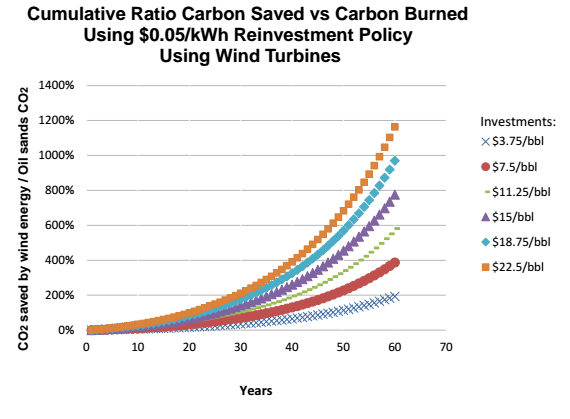
\includegraphics{g1.png} \\
{\bf Figure 1.} Amount of CO$_2$ offset by \$20/bbl investment in wind turbines based on \$4/Watt installed, and a \$0.05/kWh reinvestment from the wind power generated. This graph assumes ultimately 50\% of the total oil sands land area being reclaimed with wind turbine installations. See the spreadsheet provided in supplemental materials to investigate different costs basis scenarios.
\end{center}

\begin{center}
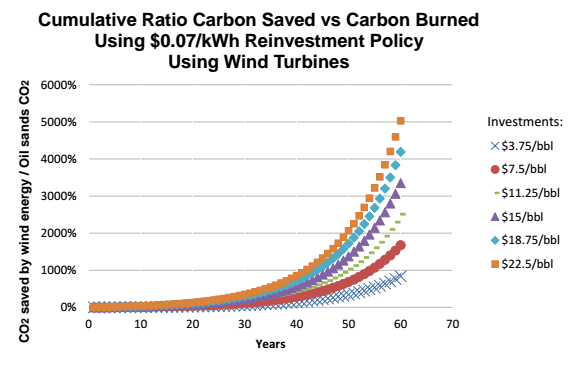
\includegraphics{g2.png}
{\bf Figure 2.} Amount of CO$_2$ offset by \$20/bbl investment in PV solar panels based on \$4/Watt installed, 15\% net system efficiency, and a \$0.05/kWh reinvestment from the solar power generated. This graph assumes 30\% of land area being reclaimed with PV solar cell installations. See the spreadsheet provided in supplemental materials to investigate different costs basis scenarios.
\end{center}

In addition to improving EROI, this proposed investment represents an alternative to a potential carbon tax because companies are investing in their own future and they benefit from the power generated.  This benefits the oil sands companies directly and immediately because they can use the electric power for production of the oil sands instead of having to build more transmission lines, or install mini nuclear reactors [5] to bring power in for which they then have to pay to use. Furthermore, once the number of turbines increases to a point, they can start sending power out on the same power lines they initially had installed to bring power in (are in the process of installing) to develop the oil sands.

%%%%%%%%%%%%%%%%%%%%%%%%%%%%%%%%%%%%%%%%%%%%%%%%%%%%%%
% 2)  Alberta Oil Sands Analysis Section
%%%%%%%%%%%%%%%%%%%%%%%%%%%%%%%%%%%%%%%%%%%%%%%%%%%%%%

\section{Alberta's Oil Sands Analysis}

\subsection{CO$_2$ Emissions Overview}

Each day, oil sands mining operations release as much CO$_2$ as all the cars in Canada [6]. In 2011, production of oil sands released an estimated of 47.1 million metric tonnes of CO$_2$ into the air [7]. Considering that in 2011, 1.8 million barrels a day were produced, Table 1 estimates the CO$_2$ emissions from oil sands production and oil use: \\

\newpage

\begin{center}
{\bf CO$_2$ from Tar Sands production and oil use} \\
\begin{tabular}{|l|l|}
\hline
\cellcolor[gray]{0.8} {\bf Production} & \cellcolor[gray]{0.8} {\bf Use} \\
\hline
Oil produced (million barrels per year) & 693.5\\
\hline
CO$_2$ to produce the oil (megatonnes/year) & 50 \\
\hline
\hspace{8.5em} CO$_2$ attributed to the mining & 0.07 \\
\hline
\hspace{1em} CO$_2$ attributed to consumption of oil sands oil & 0.43\\
\hline
CO$_2$ from oil use (megatonnes/year)  & 298.2 \\
\hline  
Total CO$_2$ from tar sands (megatonnes/year) & 348 \\
\hline
\end{tabular}
\end{center}
\begin{center}
{\bf Table 1.} Estimated total amount of $CO_2$ from Oil Sands Production and Oil Use.
\end{center}

\subsection{The Keystone XL Pipeline}
One of the biggest challenges in Alberta's Oil Sand industry is sufficient pipeline access to transport the oil to Western Canada and Southern U.S. refiners. Consequently, much of the oil is finding its way out of Alberta on trains and even trucks, which can be two or three times more expensive than pipeline costs [8]. The Keystone XL environmental review included a wide variety of cost estimates that with rail shipments to the Gulf Coast, it costs between \$15-\$20 a barrel [9]. This further justifies the investment in renewable energy systems as part of land reclamation if it helps overcome objections to the Keystone XL pipeline.\\
The Keystone XL pipeline is a major milestone in the next phase of extracting oil sands under Canada's Boreal Forest to reach higher prices of overseas markets. However, the US has yet to issue a decision on allowing the pipeline to be built as there is significant public opposition.  The projected impact of Keystone XL by the U.S Department of State in the “Final Environmental Impact Statement” (FEIS) [10] is stated as:

\begin{itemize}
\item Projected 830,000 barrels/day flow
\item An additional 147 to 168 million metric tons of greenhouse gas emissions would be annually released by the oil sands
\end{itemize}

The Canadian Association of Petroleum Producers (CAPP) 2013 Crude Oil Forecast, Markets and Transportation forecasts Canadian crude oil production will more than double to 6.7 million barrels per day by 2030 from 3.2 million barrels per day in 2012. This includes oil sands production of 5.2 million barrels per day by 2030, up from 1.8 million barrels per day in 2012 [11]. Meanwhile in the US, two senators called on the Secretary of State John Kerry and the Obama Administration to conduct “an immediate and comprehensive study" of the public health risks to communities from the proposed Keystone XL pipeline would carry diluted bitumen from Alberta across the US-Canada border to refineries on the Texas Gulf Coast [12]. \\

\emph{These opposing points of view may be resolved, we hypothesize, with the renewable electric power and long term $CO_2$ reduction that would result from the reclamation methods proposed in this paper.} \\

Another benefit of generating significant electric power in-situ from renewable resources is reduced pipeline pumping costs. It has been estimated current transport costs including extra lubricants needed to pump the thick oil through thousands of miles of pipeline add about \$18 a barrel to get oil sands crude from Western Canada down to the US Gulf Coast on the Keystone XL [8]. If plentiful electric power were available, the case could be made for at least partially refining the oil on site so lighter crude could be more easily pumped through the pipeline. \\

Furthermore, if we extend our way of thinking to include lessons from history in other related industry areas, considering the lessons of tanker ships could mitigate concerns about environmental damage from a spill.  For many years industry insisted single hull tankers were sufficient and double hull tankers too expensive, but after repeated accidents, double hull tankers have become the norm.  For a pipeline, we could borrow from landfill technology and line the trench with an impermeable membrane, and then the oil-carrying pipe would rest in a bed of sand and very course rock with drain lines along side it.  In the event of a spill the oil could be contained and rapidly pumped out.  Large tanks periodically placed along the pipeline could hold water for irrigation, or in the event of a spill, they could be rapidly emptied and used as receptacles.  Once again more symbiotic thinking could help provide solutions to our more difficult problems.

%%%%%%%%%%%%%%%%%%%%%%%%%%%%%%%%%%%%%%%%%%%%%%%%%%%%%%
% 3) Oil Sands EROI Analysis Section
%%%%%%%%%%%%%%%%%%%%%%%%%%%%%%%%%%%%%%%%%%%%%%%%%%%%%%

\section{Oil Sands EROI Analysis}

\subsection{Oil Sands EROI Overview}

Higher oil prices have boosted oil sands revenues, but operating costs have also increased significantly with the rise in energy prices. Currently the cost of production of a barrel of oil sand is in the \$40/bbl range and capital costs add another \$10-\$20/bbl [13].\\

Natural gas requirements for the oil sands industry are projected to increase to 2.1 billion cubic feet per day in 2015 [14]. Natural gas is combusted on site to fuel steam generation units to provide steam which is pumped underground to reduce the viscosity of the bitumen so it can then be more easily extracted, and the process bitumen that is mined. However, the use of natural gas exposes production to economic risk through the highly variable nature of natural gas cost. In addition, natural gas combustion for steam production is the primary source of greenhouse gas emissions for an in-situ project [15]. If natural gas prices increased to \$8/GJ, oil sands production cost would increase by \$6.30 per barrel [16].\\ 

Higher natural gas prices have encouraged companies to use natural gas more efficiently and to look for alternative fuels.  Many attempts have been made in the past to show how nuclear power may be used to supply the energy demand created by the growth of development in the oil sands regions, including installation of newly proposed Molten Salt Nuclear Reactors [15]. In 2013, there was discussion about including mini nuclear reactors from Toshiba to mine oil sands with initial deployment projected by 2020 [5].\\

Every dollar invested in the oil sands creates about 8 dollars worth of economic activity. Oil sands related investments is expected to generate 79.4 billion dollars in federal and provincial government revenues between 2012 and 2035 [30]. Oil sands investment will total hundreds of billions over the next 25 years (2012-2035) with 162.3 billion dollars to be invested in maintenance infrastructure [30]. \\

We hypothesize that a better EROI would be obtained by investing in renewable energy systems emplaced on land to be reclaimed from mining activities. In the short term, companies would be able to insert electric heaters in the ground to make the oil flow instead of having to inject steam, and at refining of the heavy oil could be done so it could be sent through the pipeline in lighter more valuable form. In the long term, it would be possible to send power generated out along the power lines that recently have been built to provide power to the oil sands region, thus enabling coal-fired power plants in the other regions to be phased out.

\subsection{CO$_2$ Offset by Investing in Wind Energy}

The installation of one 5MW wind turbine per square kilometer of reclaimed land up to a total of 70,100 square kilometers (50\% of the Alberta Oil sands area), would require an annual investment of about \$20/bbl with \$0.05/kWh reinvestment into purchasing more wind turbines.  The number of wind turbines installed would grow rapidly over the years, which would offset the CO$_2$ created by mining and using the oil sands oil in approximately 54 years. \\
 
Furthermore, it is common for the return on investment (ROI) period for a wind turbine to be about 10 years [17], which means the \$20/bbl invested is actually fully recouped in 10 years and then onward the wind turbine becomes a net income producer [17].  The turbines has a 20 year expected life, and the eventual replacement cycle would help ensure a robust wind energy business which is a source of high quality jobs. \\

Installing wind turbines in this region also need not reduce the amount of forest being replanted because the surface footprint of a large wind turbine is relatively small and tall towers enable the turbine to be placed high above the treeline Comparing the net carbon captured by the forest area of a turbine’s footprint compared to the carbon offset of a turbine, we find that the CO$_2$ captured from the boreal forest is about 26.2 tonnes/km2 [18] compared to a CO$_2$ offset by having a large wind turbine, which saves 8500 tonnes/year/MW by not burning coal to produce energy generated by wind. Therefore, there is a strong motivation for oil sands land mining reclamation to not to just replant the forest, but to plant forest and a large high hub height wind turbine every square kilometer. \\
  
There is the issue of migrating birds and local birds of prey which needs to be studied and considered; however, given the northern location, other options can be considered such as brightly coloured blades and poles to visually warn birds.  During periods of large migration, radar can be used to identify flock positions and selected turbines can be turned off.
The initial reinvestment and reclamation hypothesis appears promising, and Figures 3 and 4 show different scenarios for different percentage of investments that will need to be considered by a more detailed investigation.  Table 2 shows the modeling assumptions and Table 3 shows the years to achieve 100\% cumulative CO$_2$ offset by various investment strategies.

\begin{center}
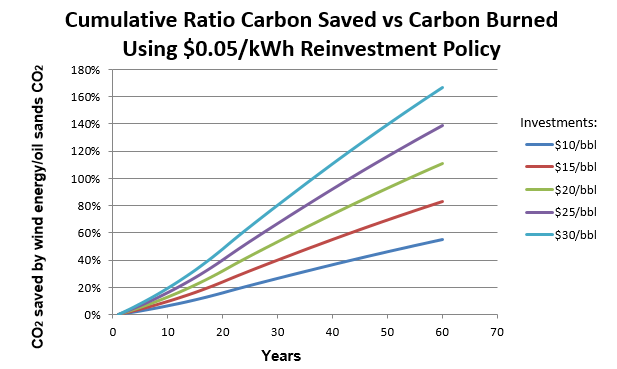
\includegraphics{g3.png}
{\bf Figure 3.} Amounts of CO$_2$ offset with different investments in Wind Energy, assuming a life expectancy of 20 years, and a \$0.05/kWh reinvestment into purchasing more wind turbines. 
\end{center}

\begin{center}
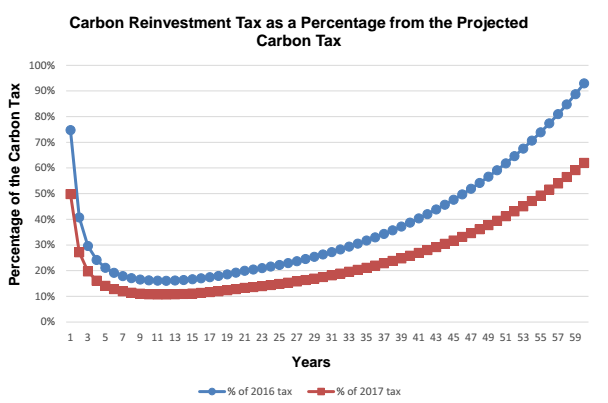
\includegraphics{g4.png}
{\bf Figure 4.} Amounts of CO$_2$ offset with different investments in Wind Energy, assuming a life expectancy of 20 years, and a \$0.07/kWh reinvestment into purchasing more wind turbines. 
\end{center}

\begin{center}
\begin{tabular}{|l|l|}
\hline
\cellcolor[gray]{0.8}{\bf Description} & \cellcolor[gray]{0.8}{\bf Value} \\
\hline
Turbine Peak Power (MW) & 5 \\
\hline
Capacity factor & 40\% \\
\hline
Land area per turbine (km$^2$) & 1 \\
\hline
Percent land area for wind turbines & 50 \% \\
\hline
area of wind farm (km$^2$) & 70,100 \\
\hline
\hspace{18em} Square miles & 27,383 \\
\hline
\hspace{12em} Square size (miles x miles) & 165 \\
\hline
Number of turbines to be built for land area & 70,100 \\
\hline
Average Power generated (GW) & 198 \\
\hline
Average annual energy produced (TWHr) & 1,734 \\
\hline 
{\bf CO$_2$ saved by wind turbines (megatonnes/year)} & {\bf 1,684} \\
\hline
\end{tabular}
\end{center}
\begin{center}
{\bf Table 2.} Modelling assumptions for determining amount of $CO_2$ saved by Wind Turbines
\end{center}

\begin{center}
\begin{tabular}{|c|c|c|}
\hline
{\bf Investment Amount} & \parbox[t]{5cm}{{\bf  Estimated Time \\ with \$0.05/kWh \\ Reinvestment}} & \parbox[t]{5cm}{{\bf Estimated Time\\  with \$0.07/kWh \\ Reinvestment}} \\
\hline
10 & 113 & 61  \\
\hline
15 & 73 & 48 \\
\hline
20 & 54 & 39.5 \\
\hline
25 & 43 & 34 \\
\hline
30 & 35 & 30 \\
\hline
\end{tabular}
\end{center}
\begin{center}
{\bf Table 3.} Estimated timeline for 100\% CO$_2$ offset for Wind Energy based on \$X/bbl and \$0.05/kWh or \$0.07/kWh Reinvestment Policy. 
\end{center}

These scenarios are dependent on three parameters: the percentage of investment per barrel of oil sand (\$/bbl), the life expectancy of wind turbines, and the reinvestment amount for new equipment (\$/kWh). If we invest the same amount each year eventually we hit a steady state for number of turbines vs. carbon emissions. The ability to achieve a 100\% offset is sensitive to the \$/kWh reinvestment from power generated. For example, with 20-year life expectancy and \$0/kWh of reinvestment we need the percentage of investment per barrel to be bigger than \$45/bbl to ultimately reach 100\% ever.  \\

Other model considerations include:

\begin{itemize}
\item {\bf Wind Turbine Peak Power}
\begin{itemize}
\item The choice of 5 MW/km$^2$ is conservative as forthcoming are 7 MW turbines, although they will require larger spacing.  Even 10 MW turbines are under consideration for production.
\end{itemize}
\item {\bf Wind Turbine Capacity Factor}
\begin{itemize}
\item NREL's median capacity factor to be 40\% for onshore wind turbines
\item With higher hub heights, up to 140m, wind turbine net capacity factor could rise to 50\%.
\end{itemize}
\item {\bf Land area per turbine}
\begin{itemize}
\item Land area assumed to cover 1 km$^2$ per turbine, many wind farms actually place up to two turbines in this area.
\end{itemize}
\item {\bf Percent land area for wind turbines}
\begin{itemize}
\item Assumption to cover 50\% of the total Alberta tar sands area
\end{itemize}
\item {\bf Reinvesment Policy}
\begin{itemize}
\item Assumption to reinvest \$0.05/kWh or \$0.07/kWh into wind turbine purchase and maintenance.
\end{itemize}
\end{itemize}

\subsection{CO$_2$ Offset by Investing in Solar Energy}

If one were to invest \$20/bbl into PV panels to create solar electric generating stations on up to 15\% of the total Oil Sand Region, assuming 30\% coverage by PV panels of the land allocated to the solar electric generating station, then this approach would in fact never totally offset the CO$_2$ created by mining and using the oil sands oil. This is due to the decommission period of the solar panels. Current panel technology and effective installation costs prevent being able to offset the CO$_2$ attributed to oil sands. However, a significant amount of CO$_2$ reduction could be accomplished and therefor the analysis of this scenario is presented here for completeness.  Figure 5 and Figure 6 show different scenarios for different percentage of investments and Table 4 presents modelling assumptions.

\begin{center}
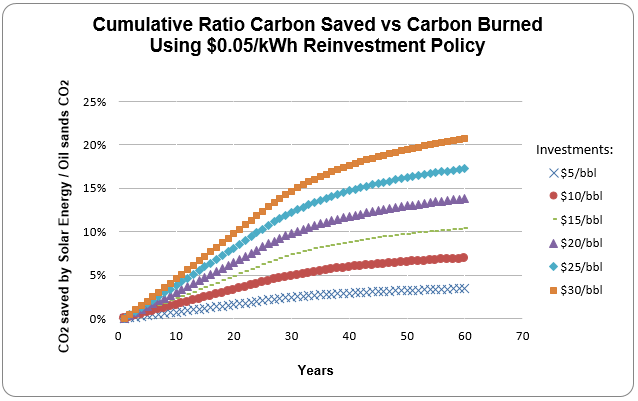
\includegraphics{g5.png}
\end{center}

\begin{center}
{\bf Figure 5.} Amounts of CO$_2$ offset with different investments in Solar Energy, assuming a life expectancy of 25 years, and a \$0.05/kWh reinvestment from the solar power generated for purchasing more solar panels.  
\end{center}

\begin{center}
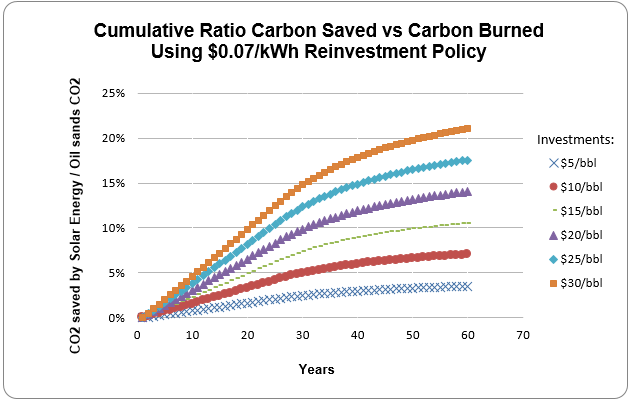
\includegraphics{g6.png}
\end{center}

\begin{center}
{\bf Figure 6.} Amounts of CO$_2$ offset with different investments in Solar Energy, assuming a life expectancy of 25 years, and a \$0.07/kWh reinvestment from the solar power generated for purchasing more solar panels.  
\end{center}

\begin{center}
\begin{tabular}{|l|c|}
\hline
\cellcolor[gray]{0.8}{\bf Description} & \cellcolor[gray]{0.8}{\bf Value} \\
\hline
Percent land area assumed covered by PV fields & 15 \% \\ 
\hline
Area of PV farm (km$^2$) & 14,020 \\
\hline
\hspace{24.5em} (Square miles) & 5,477 \\
\hline
\hspace{19em} Square Size (miles x miles) & 74 \\
\hline
Density of coverage on land designated  for PV fields & 30\% \\
\hline
Area of PV cells (m$^2$) &  6,309,000,000 \\ 
\hline
PV Cell efficiency & 15 \% \\
\hline
Average 24/7 solar insolation April (WH/m$^2$/day) &  \\
\hline
\hspace{29.5em}June & 6,250 \\
\hline
\hspace{28em}January & 1,389 \\
\hline
Average power (assumes 24/7 operation with storage technology) (GW) & \\
\hline
\hspace{29.5em}June & 164 \\
\hline
\hspace{28em}January & 37 \\
\hline
\hspace{28em}Average & 100.405 \\
\hline  
{\bf Total CO$_2$ saved by PV cells (megatonnes/year)} & {\bf 854} \\
\hline
\end{tabular}
\end{center}

\begin{center}
{\bf Table 4.} Amount of CO$_2$ saved by not burning coal to produce energy by PV solar panels
\end{center}

Similarly, the behavior of these results are controlled by the (\$/bbl) investment, the life expectancy of the solar cells, and the (\$/kWh) reinvestment into purchasing more solar cells. Other model considerations include:

\begin{itemize}
\item {\bf Percent land covered by PV fields}
\begin{itemize}
\item Assumption to be a 200W peak power solar photovoltaic panel
\end{itemize}
\item {\bf Percent land covered by PV fields}
\begin{itemize}
\item Assumption to cover 15\% of land area
\end{itemize}
\item {\bf Density of coverage on land designated for PV fields}
\begin{itemize}
\item	Assumption to cover 30\% of land area
\end{itemize}
\item {\bf Efficiency of PV fields}
\begin{itemize}
\item For this analysis, OPV efficiency was estimated to be a conservative 15\%.
\item PV cell efficiency is expected to reach 23\% by 2015 [19]
\end{itemize}
\item {\bf Reinvestment Policy}
\begin{itemize}
\item Assumption to reinvest \$0.05/kWh or \$0.07/kWh into solar equipment purchasing. This  also includes the maintenance of solar panels
\end{itemize}
\end{itemize}

The assumptions appear reasonable, but readers can investigate the results from other values using the spreadsheet provided as part of the supplemental materials. 

\subsection{CO$_2$ Offset Calculation}

The CO$_2$ offset percentage is obtained with the following formula:

\begin{displaymath}
Carbon_{offset} = \frac{Amount \;of\; CRCS \;(Cumulative \;Ration \;Carbon \;Saved)}{Amount \;of \;CB \;(Carbon\; Burned)}
\end{displaymath}

To compute the amount of CRCS (Cumulative Ration Carbon Saved):

\begin{displaymath}
CRCS_{t+1} = CRCS_t + \frac{\# (installed \;wind\; turbines)_t}{\# \;total \; turbines \; to\; build \; for \; land \; area} \times \alpha
\end{displaymath}

Where
\begin{displaymath}
\begin{split}
& \alpha =  \text{CO}_2 \;\text{saved by not burning coal to procude energy generated by wind}\\
& t \; \text{ time (in years)}
\end{split}
\end{displaymath}

To compute the standard CB (Carbon Burned) term: 
\begin{displaymath}
CB_{t+1} = \sum_{i=0}^{t} CB_t
\end{displaymath}

Where:
\begin{displaymath}
CB_t = \text{Total CO$_2$ per year from oil sands (megatonnes/year) from Table 1}
\end{displaymath}

%%%%%%%%%%%%%%%%%%%%%%%%%%%%%%%%%%%%%%%%%%%%%%%%%%%%%%
%  4) Possible Uses of Excess Power Generated Section
%%%%%%%%%%%%%%%%%%%%%%%%%%%%%%%%%%%%%%%%%%%%%%%%%%%%%%

\section{Possible Uses of Excess Power Generated}

With the availability of large amounts of electric power as more and more wind turbines come on line, the potential for revenue generation from other applications of the power increase, thereby furthering the case for investment.

\subsection{Selling Electricity Back to the Grid}

About 41\% of Alberta’s installed electricity generation capacity is from coal, 40\% from natural gas, and 8\% from wind [20]. On a long term basis, it would possible to send excess power generated by reclaimed land renewable energy systems out along same power lines that currently are bringing power into the oil sands region

\subsection{Cleaning Contaminated Water}
The Athabasca River is part of the third largest watershed in the world. Processing one barrel of bitumen requires approximately three barrels of water [6]. The contaminated water is then pumped into giant man-made tailings ponds alongside the shore with no plans for their eventual cleanup.  The contaminated water is produced from the process used to turn bitumen into diesel and other fuels. Reservoirs filled with oil sands wastewater are predicted to cover almost 62,000 acres by 2020 [21]. \\

These waters are contaminated with Polycyclic Aromatic Hydrocarbons (PAHs). These aromatic organic molecules can be hydrocracked by adding hydrogen to enable the PAHs to be turned into useful products such as plastics and pesticides. The renewable energy harvested by the wind and solar systems could be used to power the cracking process and clean up the contaminated water

\subsection{Powering Underground Electric Heaters as an Alternative to Pumping Steam Underground for Bitumen Extraction}

Another use for the excess wind power could use lessons learned from Shell Oil’s patent on installing heaters encased in pipe to liquefy the oil, so that it can be pumped to the surface [22,23]. Wind power varies with the wind, which is relatively slowly changing variable, while solar power can change suddenly with a passing cloud. In either case, to be part of a base load supply of power sent out along power lines, excess power must be stored or used immediately. The former can be accommodated over power lines with pumped storage hydro-systems or batteries. The latter is often more difficult, however underground electric heaters can often be used with greatly fluctuating power to generate heat that is diffused slowly through the ground to lower bitumen viscosity so it can flow and be extracted from wells. The nature of some underground strata gives it a very long time constant to absorb and diffuse the energy [24,25]. Where constant temperature is needed, large capacitor banks can be employed.

\subsection{Implementing UPM's Adavanced Biofuels}

Finnish company UPM is currently implementing new technology to produce wood-based biodiesel, refining the treacly residue that is left over when wood chips are cooked into pulp. This means processing husks, inedible grasses, municipal waste, and the litter from the logging industry. This technology is environmental-friendly and designed to give Europe a competitive edge in the clean energy business. \\

In research published in February, the International Council of Clean Transportation and NNFCC, a consultancy, concluded that biofuels made from waste could provide 16 per cent of Europe’s transport fuels by 2030 [27] and it would create an entirely new industry sector as current production is close to zero. In addition, the International Energy Agency (IEA) calculates that the cost of producing regular gasoline will rise from \$0.54 per litre of gasoline equivalent in 2010 to \$0.82 per litres of gasoline equivalent in 2030. By contrast, the cost of advanced biofuel production will fall from \$1.05-\$1.15 per litre of gasoline equivalent in 2010 to $0.80-$1 in 2030 [28].\\

However, the economic and societal fruits of this innovation may be harvested somewhere other than in Europe. Policy makers in Brussels are now sidelining rules on transport fuels. As a result, biofuels companies are threatening to constrain the waste-to-biofuels industry by leaving Europe for the US, China and Brazil.  \\

If UPM technology were used at oil sands to process the slash from land cleared to mine the oil sands, then this would result in a competitive diesel price, it would advance cutting-edge clean technology research in Canada, and it would significantly expand the energy ecosystem for investments in Alberta as companies are interested in harvesting their innovation somewhere other than Europe. Thus, this creates a huge profitable business for Alberta while positioning the province as a world leader in clean energy business.  


\subsection{An Alternative to a Carbon Tax}

The percentage of oil revenues to be invested (\$/bbl) into renewable energy systems as part of land reclamation efforts is a business and an environment friendly alternative to a carbon tax. Instead of paying a tax to the government, which removes value from a company ledger, this approach allows companies to invest in assets for its own present and future value, and thus could negate the perceived need by many for a carbon tax. \\

Currently, there are no tax incentives available that are specific to oil sands production. There may be industry-wide tax breaks, but they are the same for conventional oil production and for bitumen production [13]. On the other hand, the CO2-intensive nature of oil sands mining and production incites many to call for a carbon tax that could add at least \$2 to a barrel of Western Canadian heavy crude, which the US might consider as a concession to pipeline opponents in order to be able to approve the Keystone XL [8].   \\

Note there are about 0.5 tonnes of CO$_2$ that can be attributed to the mining (0.07 tonnes) and consumption (0.43 tonnes) of oil sands oil (from Table 1), and some put the cost of CO2 to be up to \$34/tonne or more [26]. If indeed as weather patterns continue to deteriorate and the latter cost were to come to be, a direct investment in renewables as an alternative to the tax would be much easier to justify. 

%%%%%%%%%%%%%%%%%%%%%%%%%%%%%%%%%%%%%%%%%%%%%%%%%%%%%%
%  5) Conclusion Section
%%%%%%%%%%%%%%%%%%%%%%%%%%%%%%%%%%%%%%%%%%%%%%%%%%%%%%

\section{Conclusion}
This paper showed that a symbiotic approach to short and long term energy needs can lead to an overall reduction in atmospheric CO$_2$. It is appears to be economical and politically prudent to undertake as soon as possible a project to install a reasonable number of wind turbines on reclaimed oil sands land in order to better investigate the hypothesis presented here to ascertain true costs, risks, and benefits with respect to ultimately widespread application of this reclamation strategy.\\

In addition, a more detailed business analysis (short and long term return of investment ROI) of the hypotheses presented here should be developed, including:

\begin{enumerate}[a)]
\item The requirement of investing a significant percentage of gross income from oil sands into renewable energy sources as part of land reclamation and to provide electricity for extracting and processing oil sands, cleaning up contaminated water, and selling excess electricity back to the grid. 
\item The time effect cost of releasing more CO$_2$ in the short term in exchange for a longer-term greater cumulative reduction in CO$_2$
\item The ability of a) above to encourage the US to approve of the Keystone XL pipeline which would save significant rail transportation costs
\item A symbiotic approach to pipeline design should also be investigated that considers using landfill liner techniques and water storage tanks normally for irrigation and as emergency spill receptacles.
\end{enumerate}

\newpage

%%%%%%%%%%%%%%%%%%%%%%%%%%%%%%%%%%%%%%%%%%%%%%%%%%%%%%
%  Bibliography Section
%%%%%%%%%%%%%%%%%%%%%%%%%%%%%%%%%%%%%%%%%%%%%%%%%%%%%%

\begin{thebibliography}{9}
\bibitem{lamport94}
 Attanasi et al.  \emph{Natural Bitumen and Extra-Heavy Oil}. Survey of energy resources (22 ed.). World Energy Council. pp. 123–140. 2010.

\bibitem{lamport94}
 \emph{About Oil Sands: Facts and Statistics.} Retrieved March 13, 2014 from
http://www.energy.alberta.ca

\bibitem{lamport94}
 \emph{Alberta's Oil Sands: Opportunity, Balance.} Government of Alberta. March 2008. Retrieved March 19, 2014 from http://environment.alberta.ca

\bibitem{lamport94}
Poisson et al.  \emph{A Time Series Analysis of Canadian Gas and Oil.} Energies 2013, 6, 5940-5959. November 2013

\bibitem{lamport94}
Daly, John.  \emph{Canada Considering Nuclear Reactors in Alberta Tar Sands Fields.} Retrieved on April 2, 2014 from http://oilprice.com 

\bibitem{lamport94}
Mettler, Peter.  \emph{Petropolis: Aerial Perspectives on the Alberta Oil Sands.}
Documentary. 2009.

\bibitem{lamport94}
Biello, David.  \emph{How Much Will Tar Sands Oil Add to Global Warming?} Retrieved on March 13, 2014 from http://www.scientificamerican.com

\bibitem{lamport94}
[8] Philips, Matthew.  \emph{Why Canada’s Oil Sands Look Like a Shaky Investment.} Retrieved on April 6, 2014 from http://www.businessweek.com/ 

\bibitem{lamport94}
Swift, Anthony.  \emph{A deeper dive: State’s environmental review of Keystone XL tar sands pipeline shows it is not in the nation’s interest.} Retrieved on April 6, 2014 from http://switchboard.nrdc.org/ 

\bibitem{lamport94}
U.S Department of State.  \emph{The Final Environmental Impact Statement (FEIS).} Retrieved from March 13, 2014 from http://keystonepipeline-xl.state.gov/

\bibitem{lamport94}
 \emph{Crude Oil Forecast, Markets \& Transportation.} Canadian Association of Petroleum Producers (CAPP). Retrieved on April 1, 2014 from http://www.capp.ca/forecast/

\bibitem{lamport94}
Prystupa, Mychaylo.  \emph{Alberta doctor tells U.S.: Canada is lying about oil sands health effects.} Retrieved Feb 27, 2014 from https://www.vancouverobserver.com/news/

\bibitem{lamport94}
Rapier, Robert.  \emph{The Cost of Production and Energy Return of Oil Sands.} Retrieved on April 1, 2014 from http://theenergycollective.com/

\bibitem{lamport94}
 \emph{Canada’s Oil Sands – Opportunities and Challenges to 2015: An Update – Questions and Answers}. Retrieved on April 2, 2014 from http://www.neb.gc.ca/ 

\bibitem{lamport94}
LeBlanc et al.  \emph{Using Molten Salt Nuclear Reactors in the Oil Sands.} 2012 World Heavy Oil Congress (WHOC’12). Aberdeen, Scotland. 2012. 

\bibitem{lamport94}
Leach, Andrew.  \emph{Rubin, oil sands, and the bitumen bubble.} Retrieved on April 6, 2014 from http://www.macleans.ca/ 

\bibitem{lamport94}
 \emph{Wind Turbine Technology.} Retrieved on April 8, 2014 from http://www.sre-tech.com/

\bibitem{lamport94}
 \emph{Carbon Sequestration Facts.} Retrieved March 19, 2014 from http://www.forestecologynetwork.org.

\bibitem{lamport94}
Kelly-Detwiler, Peter.  \emph{As Solar Panel Efficiencies Keep Improving, It's Time To Adopt Some New Metrics}. Retrieved on April 1, 2014 from http://www.forbes.com/ 

\bibitem{lamport94}
 \emph{Electricity Facts.} Retrieved on April 1, 2014 from http://www.energy.alberta.ca/ 

\bibitem{lamport94}
Loon, Jeremy Van.  \emph{ Land of Oil Lakes.} Bloomberg Businessweek November 2013, Issue 4356, p15-16.

\bibitem{lamport94}
Sandberg, Chet, Hale, Arthur, Kovscek, Anthony R.,  \emph{History and Application of Resistance Electrical Heaters in Downhole Oil Field Applications}, SPE Number SPE-165323-MS

\bibitem{lamport94}
 \emph{Shell Oil tests new oil shale technology.} Retrieved on April 6, 2014 from http://www.petroleumnews.com/ 

\bibitem{lamport94}
Closmann et al.  \emph{Method of producing shale oil from a subterranean oil shale formation.} 1970. US Patent US3501201 A

\bibitem{lamport94}
Bass et al.  \emph{Direct electric pipeline heating.} 2000. US Patent US6142707 A

\bibitem{lamport94}
 \emph{Some firms are preparing for a carbon price that would make a big difference.} Retrieved on April 8, 2014 from http://www.economist.com/

\bibitem{lamport94}
 \emph{Waste-Based Biofuels Sector Needs Smarter EU 2030 Package To Realize Its High Potential.} Retrieved on April 19, 2014 from https://www.upm.com

\bibitem{lamport94}
Oliver, Christian.  \emph{Biofuels: Wasted energy.} Retrieved on April 17, 2014 from http://ft.com

\bibitem{lamport94}
 \emph{Oil Sands 101.} Retrieved on August 20, 2014 from  http://www.energy.alberta.ca/OilSands

\bibitem{lamport94}
 \emph{Oil Sands Facts and statistics.} Retrieved on August 20, 2014 from http://www.energy.alberta.ca/OilSands
 
\end{thebibliography}

\end{document}
